%%── PANEL 6: Temas 6, 7, 8 y 9 ──────────────────────────────────────────────
\panel{LightBg}{%
  \phdr{Emerald}{6 · Densidad natural}
  \begin{tcolorbox}[def,title={Definici\'on}]
    {\scriptsize $d(A)=\limsup_{n\to\infty}\dfrac{|A\cap\{1,\ldots,n\}|}{n}$}
  \end{tcolorbox}

  \begin{tcolorbox}[key]
    {\scriptsize
    $d(n\mathbb{N})=\tfrac{1}{n}$ \quad
    $d\!\left(\{n^2\}\right)=0$ \quad
    $d(\text{primos})=0$}
  \end{tcolorbox}

  \phdr{Amethyst}{7 · Teorema de Szemer\'edi (1975)}
  \begin{tcolorbox}[pthm,title={Teorema}]
    {\scriptsize Todo $A\subseteq\mathbb{N}$ con $d(A)>0$ contiene PA de
    \textbf{cualquier} longitud finita.}
  \end{tcolorbox}
  {\scriptsize Implica VdW: en una $r$-coloraci\'on alguna clase de color
  tiene $d\geq 1/r>0$, luego contiene PA de cualquier longitud.}

  \phdr{Teal}{8 · Teorema de Green-Tao (2004)}
  \begin{tcolorbox}[ex,title={El problema}]
    {\scriptsize $d(\text{primos})=0$ $\Rightarrow$ Szemer\'edi \textbf{no
    aplica}. ?`Contienen los primos PA arbitrariamente largas?}
  \end{tcolorbox}

  \begin{tcolorbox}[tthm,title={Teorema (Green y Tao, 2004)}]
    {\scriptsize Los n\'umeros primos contienen progresiones aritm\'eticas
    de \textbf{cualquier} longitud finita $k$.}
  \end{tcolorbox}

  \begin{center}
  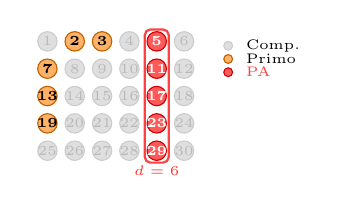
\begin{tikzpicture}[scale=0.56]
    \foreach \nnum/\px/\py in {
        1/0/0,4/3/0,6/5/0,
        8/1/1,9/2/1,10/3/1,12/5/1,
        14/1/2,15/2/2,16/3/2,18/5/2,
        20/1/3,21/2/3,22/3/3,24/5/3,
        25/0/4,26/1/4,27/2/4,28/3/4,30/5/4}{
      \filldraw[gray!25,draw=gray!40]
        ({0.62*\px},{-0.62*\py}) circle (0.22cm);
      \node[text=gray!55,font=\tiny] at ({0.62*\px},{-0.62*\py}) {\nnum};
    }
    \foreach \nnum/\px/\py in {2/1/0,3/2/0,7/0/1,13/0/2,19/0/3}{
      \filldraw[orange!60,draw=orange!75!black]
        ({0.62*\px},{-0.62*\py}) circle (0.22cm);
      \node[text=black,font=\tiny\bfseries] at ({0.62*\px},{-0.62*\py}) {\nnum};
    }
    \foreach \nnum/\px/\py in {5/4/0,11/4/1,17/4/2,23/4/3,29/4/4}{
      \filldraw[red!65,draw=red!80!black]
        ({0.62*\px},{-0.62*\py}) circle (0.22cm);
      \node[text=white,font=\tiny\bfseries] at ({0.62*\px},{-0.62*\py}) {\nnum};
    }
    \draw[red!75,thick,rounded corners=2pt]
      ({0.62*4-0.27},0.27) rectangle ({0.62*4+0.27},{-0.62*4-0.27});
    \node[red!80,font=\tiny\bfseries] at ({0.62*4},{-0.62*4-0.45}) {$d=6$};
    \filldraw[gray!25,draw=gray!40]    (4.1,-0.10) circle (0.10cm);
    \node[font=\tiny,right=1pt] at (4.22,-0.10) {Comp.};
    \filldraw[orange!60,draw=orange!75!black] (4.1,-0.40) circle (0.10cm);
    \node[font=\tiny,right=1pt] at (4.22,-0.40) {Primo};
    \filldraw[red!65,draw=red!80!black](4.1,-0.70) circle (0.10cm);
    \node[red!75,font=\tiny,right=1pt] at (4.22,-0.70) {PA};
  \end{tikzpicture}
  \end{center}
  {\scriptsize\textbf{Ej.:} $k=5$: $5,11,17,23,29$ \quad $k=6$: $7,157,\ldots,757$}

  \phdr{Navy}{9 · Conclusiones}
  {\scriptsize El hilo conductor: el orden aritm\'etico es inevitable
  incluso cuando la densidad colapsa a cero.}

  \begin{tcolorbox}[key]
    {\scriptsize\centering\bfseries
    Incluso los primos\,---\,densidad cero\,---
    no escapan al orden aritm\'etico.}
  \end{tcolorbox}
}%
